\documentclass[nooutcomes]{ximera}
%\documentclass[space,handout,nooutcomes]{ximera}

% For preamble materials

\usepackage{pgf,tikz}
\usepackage{mathrsfs}
\usetikzlibrary{arrows}
\usepackage{framed}
\usepackage{amsmath}
\pgfplotsset{compat=1.17}

\def\fixnote#1{\begin{framed}{\textcolor{red}{Fix note: #1}}\end{framed}}  % Allows insertion of red notes about needed edits
%\def\fixnote#1{}

\def\detail#1{{\textcolor{blue}{Detail: #1}}}   

\pdfOnly{\renewenvironment{image}[1][]{\begin{center}}{\end{center}}}

\graphicspath{
  {./}
  {chapter1/}
  {chapter2/}
  {chapter4/}
  {proofs/}
  {graphics/}
  {../graphics/}
}

\newenvironment{sectionOutcomes}{}{}


%%% This set of code is all of our user defined commands
\newcommand{\bysame}{\mbox{\rule{3em}{.4pt}}\,}
\newcommand{\N}{\mathbb N}
\newcommand{\C}{\mathbb C}
\newcommand{\W}{\mathbb W}
\newcommand{\Z}{\mathbb Z}
\newcommand{\Q}{\mathbb Q}
\newcommand{\R}{\mathbb R}
\newcommand{\A}{\mathbb A}
\newcommand{\D}{\mathcal D}
\newcommand{\F}{\mathcal F}
\newcommand{\ph}{\varphi}
\newcommand{\ep}{\varepsilon}
\newcommand{\aph}{\alpha}
\newcommand{\QM}{\begin{center}{\huge\textbf{?}}\end{center}}

\renewcommand{\le}{\leqslant}
\renewcommand{\ge}{\geqslant}
\renewcommand{\a}{\wedge}
\renewcommand{\v}{\vee}
\renewcommand{\l}{\ell}
\newcommand{\mat}{\mathsf}
\renewcommand{\vec}{\mathbf}
\renewcommand{\subset}{\subseteq}
\renewcommand{\supset}{\supseteq}
%\renewcommand{\emptyset}{\varnothing}
%\newcommand{\xto}{\xrightarrow}
%\renewcommand{\qedsymbol}{$\blacksquare$}
%\newcommand{\bibname}{References and Further Reading}
%\renewcommand{\bar}{\protect\overline}
%\renewcommand{\hat}{\protect\widehat}
%\renewcommand{\tilde}{\widetilde}
%\newcommand{\tri}{\triangle}
%\newcommand{\minipad}{\vspace{1ex}}
%\newcommand{\leftexp}[2]{{\vphantom{#2}}^{#1}{#2}}

%% More user defined commands
\renewcommand{\epsilon}{\varepsilon}
\renewcommand{\theta}{\vartheta} %% only for kmath
\renewcommand{\l}{\ell}
\renewcommand{\d}{\, d}
\newcommand{\ddx}{\frac{d}{dx}}
\newcommand{\dydx}{\frac{dy}{dx}}


\usepackage{bigstrut}


%\usepackage{tikz}


\title{Measurement}
\author{Brad Findell}
\begin{document}
\begin{abstract}
Short-answer problems about measurement. 
\end{abstract}
\maketitle



%\textbf{Definition.} Under a \textbf{dilation} about center $O$ and scale factor $r>0$, the image of $P$ is 
%a point $Q$ so that $Q$ lies on \wordChoice{\choice{segment}\choice[correct]{ray}\choice{line}} 
%$\answer[format=string]{OP}$ % $\overrightarrow{OP}$ 
%and $OQ=\answer[format=string]{rOP}$.  The image of $O$ is $\answer[format=string]{O}$. 

\section{Numbers, Units, and Quantities}
In this section, we develop and explain the algebra of measurement calculations and unit conversions. 

\begin{question}
Brad measured his driveway to be 21 feet long.  How long is it in yards?  
$\answer{7}$ yards.  
\end{question}

We all know that 3 feet and 1 yard express the same length.  Let's write an equation to express this equality of lengths: 
\[
3\;\textrm{ft} = 1\;\textrm{yd}
\]

Here is a picture illustrating this idea:  

\begin{image}
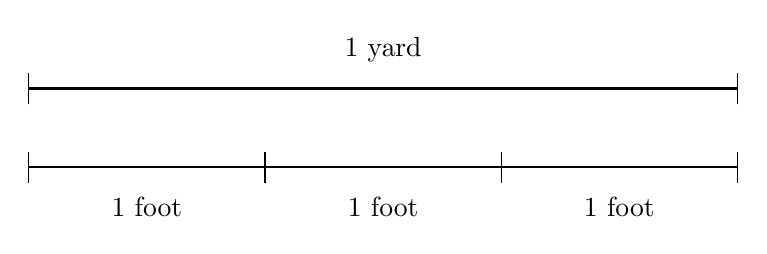
\begin{tikzpicture}[xscale=1]
\draw [thick] (0,1) -- (9,1);
\draw (0,1-.2) -- (0, 1+.2);
\draw (9,1-.2) -- (9,1+ .2);
\draw [thick] (0,0) -- (9,0);
\draw (0,-.2) -- (0, .2);
\draw (3,-.2) -- (3, .2);
\draw (6,-.2) -- (6, .2);
\draw (9,-.2) -- (9, .2);
\node[align=center] at (4.5,1.5)%
{1 yard};
\node[align=center] at (1.5,-.5)%
{1 foot};
\node[align=center] at (4.5,-.5)%
{1 foot};
\node[align=center] at (7.5,-.5)%
{1 foot};
\end{tikzpicture}
\end{image}

\begin{question}
The equation $3\;\textrm{ft} = 1\;\textrm{yd}$ seems to suggest that you \wordChoice{\choice[correct]{multiply}\choice{divide}} feet by 3 to get yards.  But when converting feet to yards in the question above you \wordChoice{\choice{multiplied}\choice[correct]{divided}} the number of feet by 3.  

Why do these answers appear to be opposites of each other?  
\end{question}

The resolution of this conundrum requires that we distinguish numbers (e.g., 21) from units (e.g., feet).  Quantities measuring, say, length, weight, or speed involve both numbers and units, but the numbers behave differently from the units, as we see in the example above.  

With a little algebraic manipulation, the equation $3\;\textrm{ft} = 1\;\textrm{yd}$ is equivalent to the following equations:  
\[
\frac{3\;\textrm{feet}}{1\;\textrm{yard}} = 1\qquad \textrm{and}\qquad \frac{1\;\textrm{yard}}{3\;\textrm{feet}} = 1.
\]
In both equations, the 1 on the right is ``dimensionless'' in the sense that it is without units.  Think of it as a scale factor of 1, which leaves lengths unchanged.  These equations are useful for demonstrating the conversion from feet to yards and vice versa:  

%\begin{align*}
%21\textrm{ feet} &= 21\; \textrm{feet} \\
%21\textrm{ feet} &= 21\textrm{ feet} \\
%21\textrm{ feet} &= 21\ \textrm{feet} \\
%21\textrm{ feet} &= 21\, \textrm{feet} \\
%21\textrm{ feet} &= 21\: \textrm{feet} 
%\end{align*}

\[
21\;\textrm{feet} = 21\;\cancel{\textrm{feet}} \cdot \frac{{1\;\textrm{yard}}}{3\;\cancel{\textrm{feet}}} = 7\;\textrm{yards}
\]

\[
7\;\textrm{yards} = 7\;\cancel{\textrm{yards}} \cdot \frac{{3\;\textrm{feet}}}{1\;\cancel{\textrm{yard}}} = 
21\;\textrm{feet}
\]

These examples illustrate an \emph{algebra of units}, in which units behave much like algebraic variables.  In both conversions, we multiply a quantity by a dimensionless 1, so that the calculation doesn't change the amount that the quantity represents.  The cancellation of units helps to confirm that we are doing the calculation correctly.  

At a conceptual level, this algebra of units helps illuminate how the numbers and units behave in apparently opposite ways:  

\begin{itemize}
\item Yards are three times as big as feet, so there are one-third as many in a given length.  
\item Feet are one-third the size of yards, so there are three times as many in a given length.  
\end{itemize}

Thus, we must be careful to consider whether the letters represent numbers or units.  

Let's try another problem.  

\begin{question}
At Big State University, the student-professor ratio is 8 to 1.  Write an equation relating the number of students, $s$, to the number of professors, $p$.  

Answer:  $s = \answer{8p}$.  
\end{question}

In response to this question, it is tempting to write $8s = p$ or its equivalent, $s=p/8$, and these turn out to be very common incorrect answers among students.  But let's try some specific numbers:  If there are 160 students, then there should be 20 professors, but the equation says that $p = 8s = 8\cdot 160 = 1280$, which would mean 1280 professors.  Clearly the equation is backwards: It caused us to multiply the number of students by 8 when we should have divided.  

But here is another way of thinking about this incorrect answer.  If ``students'' and ``professors'' were units (like yards and feet), then the equation would be correct. Here is a picture to help:  

\begin{image}
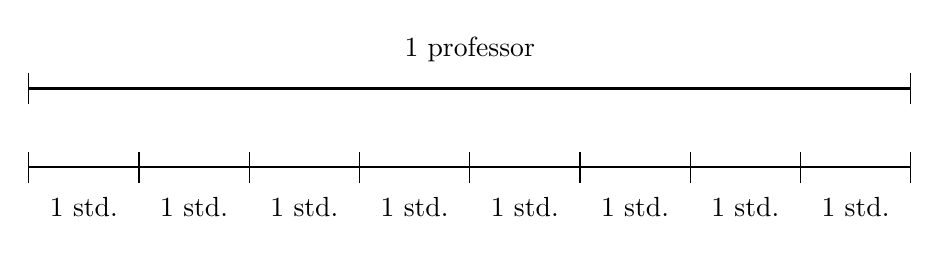
\begin{tikzpicture}[xscale=.7]
\draw [thick] (0,1) -- (16,1);
\draw (0,1-.2) -- (0, 1+.2);
\draw (16,1-.2) -- (16,1+ .2);
\draw [thick] (0,0) -- (16,0);
\draw (0,-.2) -- (0, .2);
\draw (2,-.2) -- (2, .2);
\draw (4,-.2) -- (4, .2);
\draw (6,-.2) -- (6, .2);
\draw (8,-.2) -- (8, .2);
\draw (10,-.2) -- (10, .2);
\draw (12,-.2) -- (12, .2);
\draw (14,-.2) -- (14, .2);
\draw (16,-.2) -- (16, .2);
\node[align=center] at (8,1.5)%
{1 professor};
\node[align=center] at (1,-.5)%
{1 std.};
\node[align=center] at (3,-.5)%
{1 std.};
\node[align=center] at (5,-.5)%
{1 std.};
\node[align=center] at (7,-.5)%
{1 std.};
\node[align=center] at (9,-.5)%
{1 std.};
\node[align=center] at (11,-.5)%
{1 std.};
\node[align=center] at (13,-.5)%
{1 std.};
\node[align=center] at (15,-.5)%
{1 std.};
\end{tikzpicture}
\end{image}

If professors and students are units of measurement with this consistent relationship between them, then to ``convert''  20 professors to students, we proceed just as we converted yards to feet:  

\[
20\;\textrm{professors} = 20\;\cancel{\textrm{professors}} \cdot \frac{{8\;\textrm{students}}}{1\;\cancel{\textrm{professor}}} = 
 160\;\textrm{students}
\]

The above question states, however, that the letters are to be the \emph{numbers} of students and professors, not units of measurement.  So let's repeat the previous calculation generally, with $p$ representing the number of professors and $s$ representing the number of students:  
\[
p\;\textrm{professors} = p\;\cancel{\textrm{professors}} \cdot \frac{{8\;\textrm{students}}}{1\;\cancel{\textrm{professor}}} = 
 8p\;\textrm{students} = s\;\textrm{students}
\]

So the correct equation is indeed $s = 8p$.  But again, notice how the numbers and the units work in apparently opposite ways.  

Because of the common confusion between numbers and units, some mathematics educators recommend against using the first letter of a unit to indicate the number of that unit in a measurement.  Indeed, the expressions ``$p$ professors'' and ``$s$ students'' are hard to read and interpret---and ``$8p$ students'' might be worse.  

Whether you accept this recommendation or not, here is some good advice:  
\begin{itemize}
\item When making calculations with quantities that include units, be very clear and careful about whether the letters represent units or numbers.  
\item When writing equations, it is very easy to get the relationships backwards, so check the equations with easy numbers.  
\end{itemize}

Math teachers benefit from knowing conversions from memory.  Here are some that you might not know:  

\begin{align*}
%1\;\textrm{ft} &= 12\;\textrm{in} \\
%1\;\textrm{yd} &= 3\;\textrm{ft} \\
%1\;\textrm{mile} &= 1760\;\textrm{yds} \\
1\;\textrm{mile} &= 5280\;\textrm{feet} \\
%1\;\textrm{tablespoon} &= 3\;\textrm{teaspoons} \\
%1\;\textrm{(fluid) ounce} &= 2\;\textrm{tablespoons} \\
%1\;\textrm{cup} &= 8\;\textrm{ounces} \\
%1\;\textrm{quart} &= 4\;\textrm{cups} \\
%1\;\textrm{gallon} &= 4\;\textrm{quarts} \\
%1\;\textrm{ml}  &= 1\;\textrm{cubic cm} \\
1\;\textrm{inch} &= 2.54\;\textrm{cm (exactly)} \\
1\;\textrm{kg} &\approx 2.205\;\textrm{lbs}\\
%1\;\textrm{year} &\approx 365.2425\;\textrm{days}
\end{align*}

And here is a useful uncommon conversion that makes use of common ones: 
%\[
%60 \;\textrm{mph} = \frac{60\;\textrm{miles}}{1\;\textrm{hour}} 
%=  \frac{60\;\textrm{miles}}{1\;\textrm{hour}} \cdot \frac{1\;\textrm{hour}}{3600\;\textrm{sec}} \cdot 
%\frac{5280\;\textrm{feet}}{1\;\textrm{mile}} = \frac{88\;\textrm{feet}}{1\;\textrm{sec}} = 88 \;\textrm{fps}
%\]

\[
60\;\textrm{mph} = \frac{60\;\textrm{miles}}{1\;\textrm{hour}} 
=  \frac{60\;\cancel{\textrm{miles}}}{1\;\cancel{\textrm{hour}}} \cdot \frac{1\;\cancel{\textrm{hour}}}{3600\;\textrm{sec}} \cdot 
\frac{5280\;\textrm{feet}}{{1\;\cancel{\textrm{mile}}}} = \frac{88\;\textrm{feet}}{1\;\textrm{sec}} = 88\;\textrm{fps}
\]

\begin{question}
Use the conversions above to convert 1 meter to inches and to yards. 

\[
1\;\textrm{meter} = \answer[tolerance=.01]{100/2.54}\;\textrm{inches} = \answer[tolerance=.01]{100/2.54/36}\;\textrm{yards}
\] 

\end{question}

\begin{question}
College and school tracks used to be 1/4 mile around, or 440 yards, so that a half-mile race was two laps, and a one-mile race was four laps.  Today, most college and school tracks have been converted to metric, with one lap measuring 400 meters, which is close to 440 yards.  In high-school track, the ``mile'' is usually run as 1600 meters.  

The 1600 meters race is $\answer[tolerance=.01]{10.2187}$ yards \wordChoice{\choice[correct]{shorter}\choice{longer}} than 1 mile.  

A four-minute miler should run 1600 meters about $\answer[tolerance=.05]{1.4}$ seconds (to the closest 0.05 seconds) \wordChoice{\choice[correct]{faster}\choice{slower}} than four minutes.  
\end{question}


\section{Square Units and Cubic Units}
Because $3\;\textrm{ft} = 1 \;\textrm{yd}$, it is tempting to conclude that $3\;\textrm{square feet} = 1 \;\textrm{square yards}$.  But \dots

\begin{question}
What is a square foot?  What is a square yard? 
\begin{freeResponse}
\begin{hint}
A square foot is the area of a square that measures 1 foot by 1 foot.  A square yard is the area of a yard that measures 1 yard by 1 yard. 
\end{hint}
\end{freeResponse}
\end{question}

\begin{question}
How many square feet are in a square yard?  $\answer{9}$.  

Provide a geometric explanation. Provide an explanation based on the algebra of units. 
\begin{freeResponse}
\begin{hint}
From pictures of a square yard and a square foot, it is not hard to see that it takes 9 square feet to cover 1 square yard.  (Draw pictures.)
\end{hint}
\begin{hint}
\[
1\;\textrm{square yard} = 1\;\textrm{yard}^2 = 1\cdot(3\;\textrm{feet})^2 = 9\;\textrm{feet}^2 = 9\;\textrm{square feet}
\]
\end{hint}
\end{freeResponse}
\end{question}

\begin{problem}
Convert 25 yards to meters (and 25 meters to yards) using ``2.54 cm in each inch'' as the only Metric-English unit conversion.  Now convert 25 square yards to square meters and 25 square meters to square yards.  Do the same with cubic yards and cubic meters.

$25\;\textrm{yards} = \answer[tolerance=.01]{(25)(36)(.0254)} \;\textrm{meters}$

$25\;\textrm{meters} = \answer[tolerance=.01]{2500/2.54/36} \;\textrm{yards}$

$25\;\textrm{square yards} = \answer[tolerance=.01]{25((36)(.0254))^2} \;\textrm{square meters}$

$25\;\textrm{square meters} = \answer[tolerance=.01]{25(100/2.54/36)^2} \;\textrm{square yards}$

$25\;\textrm{cubic yards} = \answer[tolerance=.01]{25((36)(.0254))^3} \;\textrm{cubic meters}$

$25\;\textrm{cubic meters} = \answer[tolerance=.01]{25(100/2.54/36)^3} \;\textrm{cubic yards}$

\end{problem}


\end{document}
